%% LyX 2.0.2 created this file.  For more info, see http://www.lyx.org/.
%% Do not edit unless you really know what you are doing.
\documentclass[noae]{article}
\usepackage[T1]{fontenc}
\usepackage[utf8x]{inputenc}
\usepackage{geometry}
\geometry{verbose,tmargin=2.5cm,bmargin=2.5cm,lmargin=2cm,rmargin=1.5cm,headsep=0.5cm,footskip=1cm}
\usepackage{amsmath}
\usepackage{amssymb}
\usepackage{graphicx}

\makeatletter

%%%%%%%%%%%%%%%%%%%%%%%%%%%%%% LyX specific LaTeX commands.
%% Because html converters don't know tabularnewline
\providecommand{\tabularnewline}{\\}

%%%%%%%%%%%%%%%%%%%%%%%%%%%%%% User specified LaTeX commands.
\batchmode

\def\input@path{{/home/tran/Bureau/miparcours//}}







%%%%%%%%%%%%%%%%%%%%%%%%%%%%%% LyX specific LaTeX commands.
%% Because html converters don't know tabularnewline
\providecommand{\tabularnewline}{\\}

%%%%%%%%%%%%%%%%%%%%%%%%%%%%%% Textclass specific LaTeX commands.
\newenvironment{lyxlist}[1]{\begin{list}{}
{\settowidth{\labelwidth}{#1}
 \setlength{\leftmargin}{\labelwidth}
 \addtolength{\leftmargin}{\labelsep}
 \renewcommand{\makelabel}[1]{##1\hfil}}}{\end{list}}



\usepackage{Sweave}

\makeatother

\begin{document}

\title{\textbf{Rapport d'avancement à mi-parcours}}


\title{\textbf{Modélisation, Simulation multi-niveau pour l'optimisation
de politiques de vaccination}}

\maketitle
\textbf{Phd: TRAN Thi Cam Giang }

\textbf{Thesis direction: Yann Chevaleyre (PR, Université Paris 13),
Jean-Daniel Zucker (DR1, UMI UMMISCO, IFI-MSI, IRD)}

\textbf{Co-supervision: Marc Choisy (CR1, MIVEGEC, NIHE, IRD), Vu
Dinh Thiem (NIHE)}


\section{Introduction}

This thesis is taking place in a context where many public health
serious events have occurred in the world : SRAS in 2003, avian influenza
in 2004 or swine flu in 2009.\textbf{ }In particular, in the start
of the 2014, the World Health Organization (WHO) had officially to
state global measles epidemic outbreak. In the first three months
of the year 2014, there were about 56,000 cases of measle infections
in 75 countries \cite{WHO2014a}, in particular in southeast Asia
particularly, in Vietnam \textbf{\cite{http://healthmap.org/site/diseasedaily/article/measles-reemerges-vietnam-22814}}.\textbf{
}This has pointed out the important role of the epidemiological phenomena
anticipation when diseases occur. Moreover, for vaccination policies,
the mass policy (vaccinate the maximum number of children before certain
age) is the oldest (started from the 1950s in the rich countries)
and is now the most used. The problem of this vaccination policy is
too expensive, ineffective and quite impossible to implement in poor
countries, especially in Africa as both financial and logistical problems.
(e.g. the WHO project ``Extended Programm on Immunization'' in Vietnam
for the measles extinction before 2012 is failed). In addition, when
a vaccination policy is performed in a country, there is only one
policy, but in modelation, we can realize many policies and at the
same time estimate them. Therefore, optimize the vaccination policies
in Artificial Intelligence in order that these policies may become
more effective, less expensive, and take into account the spatial
dimension, is the goal of this thesis.

To carry out this goal, the first task is to make a state of the art
covering the different epidemic models being used in the field of
epidemiological modeling. In the second step, we will focus on design
or expanse for representation language that allows modelers to express
the goals of model simulations as well as constraints related to them.
In the third step, we will concetrate on stochastic models, and investigate
disease spread caracteristics between population and community in
a spatial context. We then study local/global disease persistence,
disease periodicity and the influence of space on the disease persistence.
Finally, we will perform vaccination policies in a metapopulation
and optimize them bu using reinforcement learning algorithms 


\section{Epidemic models}


\subsection{Epidemic model}

It is known that, there are many current models that are used to model
complex systems in nature, in ecology system and in epidemiology.
Mathematical models in epidemiology are a typical exemple. These models
permit us to present behavior of diseases and disease process in mathematics.
They have given us good results in mathematics as deterministic models
in which every set of variable states is only determined by parameters
in the model and by sets of previous states of these variables. In
detail, the deterministic models are equations, for that they perform
the same way for a given set of initial conditions. But they don't
have randomness, dynamics, and don't present dynamic of diseases in
nature. Thus, stochastic models have been proposed. A sotchastic model
is always more realistic than a deterministic one. These models have
stochastic and variable states are not described by unique values,
but by probability distributions. It is reason for that, we will use
the stochastic models to predict extinction propability of disease
in spatial context\cite{KeelingRohani2008}. 

To present the process of infection propagation in community, we give
here the development of epidemic models by focusing on acute infections,
assuming the pathogen causes illness for a periods of time followed
by (typically lifelong) immunity. The first simplest model is the
S-I-R model created by W. O. Kermack and A. G. McKendrick in 1927.
The authors categorized hosts within a population as Susceptible (if
not yet exposed to the pathogen), Infected (if currenly infected by
the pathogen) and Recovered (if they have successfully cleared the
infection). From the simplest SIR model, in order to accord each infectious
disease and real property of disease, scientists have modified it,
made it different multiforme. However, in shape of this thesis, we
concentrate on the SEIR model (as the figure \ref{fig:seirmodel})
that fit many currently infectious diseases in the world. Each patient
must pass four steps : susceptible stage, incubation stage, infectious
stage and recovered stage.

\begin{figure}[tbph]
\centering 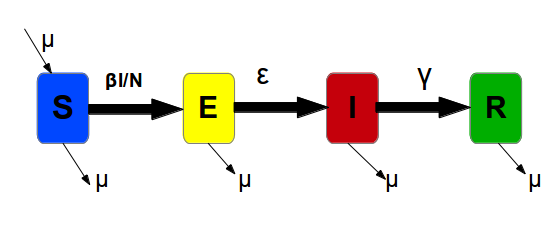
\includegraphics[width=0.3\textwidth]{seirmodel} \caption{SEIR model}


\label{fig:seirmodel} 
\end{figure}


\textbf{In this model, the host population (N) is divided into four
classes : susceptible S(t), exposed E(t), infected I(t) and recovered
R(t). We have :}

\textbf{$N(t)=S(t)+E(t)+I(t)+R(t)$ (sua cai hinh)}
\begin{itemize}
\item Classe S(t) : contains the number of individuals not yet with the
disease at time t, or those susceptible to the disease. 
\item Classe E(t) : contains the number of individuals who are in the exposed
or latent period of the disease. 
\item Classe I(t) : contains the number of individuals who have been infected
with the disease and are capable of spreading the disease to those
in the susceptible category. 
\item Classe R(t) : contains the number of individuals who have been infected
and then removed from the disease, either due to immunization or due
to death. Individuals of this classe are not able to be infected again
or to transmit the disease infection to others. 
\end{itemize}
The conceptual descriptions of the model can be represented by a flow
diagram above. The flow diagram for the SEIR model uses arrows to
present the movement between the S and I classes, the E and I classes
and the I and R classses. Here, individuals are born susceptible,
die at a rate $\mu$, become infected with the force of infection
$\lambda$ that is a function among the contact rate $\beta$, the
number of infected invidual I and the population size N, infectious
after a latency period of an average duration of $1/\sigma$ and recover
at the rate $\gamma$.


\subsection{Demographic stochasticity}

Demographic stochasticity is considered as fluctuation in population
processes that are based the random nature of events at the level
of the individual. Each event is related to one baseline probability
fixed, individuals are presented in differing fates due to chance.
In addition to the demographic stochasticity, the number of infectious,
susceptible, exposed and recovered individuals is now required to
be an interger. Modeling approches that incorporate demographic stochasticity
are called event-driven methods. These methods require explicit consideration
of events. The first method\textbf{ }\textquotedbl{}First Reaction
Method” is born in 1976 by Gillespie. Then, according to this first
method and these two key factors of demographic stochasticity models
(event, randomness) , many scientists have improved the first method,
and created many better algorithms for stochastic simulations. There
are two main types of methods, exact methods and approximative methods.
The typical approche in exact methods most practitioners use, is the
algorithm “Direct Method” of Gillespie(1977) improved from the first
approche “First Reaction Method”, and in approximative methods, is
the “tau-leaping” method.

For the Direct Method (Gillespie 1977), the first step estimates the
time until the next event, by cumulating the rates of all possible
events. Then, by transforming event rates into propabilities, the
method randomly selects one of these events. The time and numbers
in each class are then updated according to which event is chosen.
We repeate this process to iterate model through time.

For the ``tau-leaping'' method, the main crux is the use of Poisson
random variables to approximate the number of occurrences of each
type of reaction event during a carefully selected time period, $\tau$\textbf{.}

According to these two types of algorithms, the common point is both
methods use continuous-time Markov process for which the transition
rates are constants, isn't a function of time. The future state of
the process, is only conditional on the present state, but independent
of the past. 

However, for the exact algorithm, its advantage give us a really exact
approach to simulate time-to-event model. This process is repeated
to iterate the model. Gibson \& Bruck(2000) \cite{KeelingRohani2008}
modified the first reaction method and created the Next Reaction method
that substantially more challenging to program but is significantly
faster than even the method when there are a large number of different
event types. The Direct, First Reaction and Next Reaction methods
are all exact stochastic approaches of the underlying ordinary differential
equations. But, its disavantages are 1) noise in exact simulations
only affects the probabilities associated with fates of individuals
and the updating of each consecutive event is independent – there
is no assumption concerning environmental stochasticity; 2) these
exact solutions become too slow and impractical when any one transition
rate is large, when there is a big number of subpopulations or one
a big number of event in a metapopulation. It is the reason for that,
approximate models have been proposed instead of the exact stochastic
methods. Gillespie (2001) has proposed a new method that decreases
the simulation accuracy, but increases simulation speed. This is the
“tau-leap method” known as an approximate method reduces the number
of iterations by treating transition rates as constant over time periods
for which this approximation leads to little error \cite{KeelingRohani2008}
as mentioned above. However, when we use the “tau-leap method”, there
is a possibility, the number of indivudal in each class can become
negative. View the figure about simulation speed of methods \ref{fig:speed}\cite{KeelingRohani2008}.

\begin{figure}[tbph]
\centering 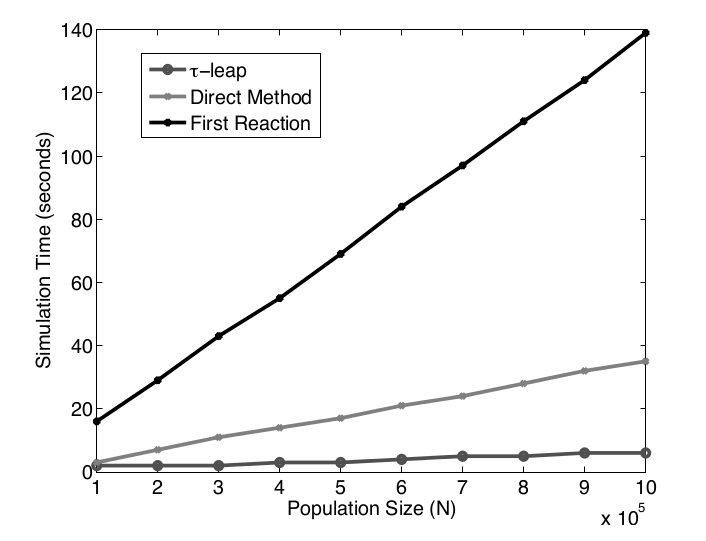
\includegraphics[width=0.5\textwidth]{speed} \caption{Figure is extrait from Keeling (2008) The time (in seconds) to simulate
1000 years of SEIR epi- demics ($\mu=0.02$ per year, $1/\sigma=8$
days, $1/\gamma=10$ days) on a 3.4GHz Pentium PC. For Gillespie’s
Direct (light grey line) and First Reaction (black line) methods,
as the population size increases so does the simulation time, which,
for very large populations, could become prohibitive. In contrast,
the ``$\tau-leap$ method (dark grey) is fast and largely unaffected
by population size \cite{KeelingRohani2008}. }


\label{fig:speed} 
\end{figure}


According this figure \textbf{\ref{fig:speed}, }when the population
size increases, the simulation time of the three methods (First Reaction,
Direct Method, $\tau-leap$) is almost augmented. The simulation time
of the method ``First Method'' is maximum, it means that this is
the slowest method, but the simulation time of the method ``$\tau-leap$''
is minimum or the fastest.\textbf{ }In the shape of my thesis, we
will use the direct method to exactly estimate spread of diseases
in metapopulation. Because the direct method is one exact approach
and its simulation time isn't too slow and too fast. Afterward, we
will use the approximate method to explore vacination policies.


\section{Approaches in use}


\subsection{Deterministic model for many cities}


\subsubsection{Deterministic model for many cities}

In modeling of ecological system, presenting interactions between
humans, subpopulations and geographic conditions, the metapopulation
model is a good choice. Metapopulation is a set of subpopulations
with mutual interaction \cite{Levins1969} here a subpopulation can
only go extinct locally and be recolonized by another after it is
emptied by extinction \cite{Bolker1996,Hanski1998,Levins1969}. In
the epidemic models, the standard SEIR model (susceptible-exposed-infective-recovered)
has been strongly developped for the dynamics of directly infectious
disease \cite{Bolker1995}. For disease-based metapopulation models,
we give here a suitable new version of the SEIR equation that would
be as follows:

Consider a metapopulation of $n$ sub-populations. In a subpopulation
$i$ of size $N_{i}$, disease dynamics can be deterministically described
by the following set of differential equations \cite{Anderson&May1992}:

\begin{eqnarray}
\frac{dS_{i}}{dt} & = & \mu N_{i}-\lambda_{i}S_{i}-\mu S_{i}\label{eq:dS}\\
\frac{dE_{i}}{dt} & = & \lambda_{i}S_{i}-\mu E_{i}-\sigma E_{i}\\
\frac{dI_{i}}{dt} & = & \sigma E_{i}-\mu I_{i}-\gamma I_{i}\label{eq:infectieux}\\
\frac{dR_{i}}{dt} & = & \gamma I_{i}-\mu R_{i}\label{eq:dR}
\end{eqnarray}
 where $S_{i}$, $E_{i}$, $I_{i}$ et $R_{i}$ are the numbers of
susceptible, exposed, infectious and recovered in this sub-population
$i$ respectively. Individuals are born susceptible, die at a rate
$\mu$, become infected with the force of infection $\lambda_{i}$,
infectious after a latency period of an average duration of $1/\sigma$
and recover at the rate $\gamma$.


\subsubsection{Formula for force of infection}

The force of infection depends not only on the total population size
$N_{i}$ and the number of infected $I_{i}$ in subpopulation $i$,
but also in other sub-populations \cite{KeelingRohani2008}.

\begin{equation}
\lambda_{i}=\beta_{i}\frac{I_{i}}{N_{i}}+\sum_{\substack{j=1\\
j\neq i
}
}^{n}\rho_{ij}\left[\frac{\beta_{i}\text{[}(1-\varepsilon_{ij})I_{j}-I_{i}]}{N_{i}}+\frac{\varepsilon_{ij}\beta_{j}I_{j}}{N_{j}}\right]\label{eq:force-1}
\end{equation}
 where $\beta_{i}$ is the contact rate in population $i$ and $\rho_{ij}=\rho_{ji}$
($0\leqslant\rho_{ij}\leqslant1$ and $\rho_{ii}=1$) is the coupling
between subpopulations $i$ and $j$. Among the infections caused
by contacts with infected from other subpopulations, $\varepsilon_{ij}=\varepsilon_{ji}$
($0\leqslant\varepsilon_{ij}\leqslant1$) is the proportion of infections
due to susceptible individuals visiting other populations as opposed
to infected individuals from other populations visiting the focal
population. See appendix for detail on the construction of this equation.
We can verify that in the limit case on one single subpopulation in
the metapopulation ($i=j$ and $n=1$) we have 
\begin{equation}
\lambda_{i}=\beta_{i}\frac{I_{i}}{N_{i}}.
\end{equation}
 Consider that the contact rate $\beta_{i}$ is seasonally forced
\cite{Altizer2006} and seasonality is an annually periodic function
of time \cite{Grenfell1995}. As a result, 
\begin{equation}
\beta_{i}(t)=b_{0}\left[1+b_{1}\cos\left(\frac{2\pi t}{T}+\varphi_{i}\right)\right]\label{eq:beta_i}
\end{equation}
 where $t$ is the time, $b_{0}$ and $b_{1}$ are the mean value
and amplitude of the infection rate $\beta$ at which susceptible
individuals become infected, $T$ and $\varphi_{i}$ are the period
and the phase of the forcing. With the annual sinusoidal form of the
infection rate, we really have the sinusoidally forced SEIR metapopulation
model.


\subsubsection{Equilibrium values of the system}

In a case the infectious contact rate is constant, the equilibrium
values of the variables $S$, $E$, $I$ and $R$ can be expressed
analytically as follows. We know that, in simulation, the equilibrium
state allow a disease to persist in a population for a long time.
So, an infectious disease in the $subpopulation_{i}$ is available
in long term this system is at equilibrium. It means that at which
$\frac{dS_{i}}{dt}=\frac{dE_{i}}{dt}=\frac{dI{}_{i}}{dt}=\frac{dR{}_{i}}{dt}=0$
({*}). Thus, we let all equations (equations $1$ - $4$ ) in the
system be equal to zero, then calculate the values of the variables
(now denoted by $S_{i}^{*}$, $E_{i}^{*}$, $I_{i}^{*}$ , and $R{}_{i}^{*}$)
that satisfy this condition ({*}). We have these values as folllows:

\begin{eqnarray}
S_{i}^{*} & = & N_{i}\frac{(\gamma+\mu)(\sigma+\mu)}{\beta\sigma}\\
E_{i}^{*} & = & N_{i}\mu\left(\frac{1}{\sigma+\mu}-\frac{\gamma+\mu}{\beta\sigma}\right)\\
I_{i}^{*} & = & N_{i}\mu\frac{\beta\sigma-(\sigma+\mu)(\gamma+\mu)}{\beta(\sigma+\mu)(\gamma+\mu)}\\
R_{i}^{*} & = & N_{i}-S_{i}^{*}-E_{i}^{*}-I_{i}^{*}
\end{eqnarray}


Here, if we set $R_{0}=\frac{\beta\sigma}{(\gamma+\mu)(\sigma+\mu)}$,
so we have

\begin{eqnarray}
S_{i}^{*} & = & N_{i}\frac{1}{R_{0}}\\
E_{i}^{*} & = & N_{i}\frac{\mu\sigma}{R_{0}}\left(R_{0}-1\right)\\
I_{i}^{*} & = & N_{i}\frac{\mu}{\beta}(R_{0}-1)\\
R_{i}^{*} & = & N_{i}-S_{i}^{*}-E_{i}^{*}-I_{i}^{*}
\end{eqnarray}


One nomal conditions for all population availabes is that the equilibrium
values cannot be negative. Therefore, an infectious disease is available
in the $subpopulation_{i}$ if $R_{0}>1$. Now, the endemic equilibrium
in the system is given by $(S_{i}^{*},E_{i}^{*},I{}_{i}^{*},R{}_{i}^{*})$
= $(N_{i}\frac{1}{R_{0}}$, $N_{i}\frac{\mu\sigma}{R_{0}}\left(R_{0}-1\right)$,
$N_{i}\frac{\mu}{\beta}(R_{0}-1)$, $N_{i}(1-\frac{1}{R_{0}}-\frac{\mu\sigma}{R_{0}}\left(R_{0}-1\right)-\frac{\mu}{\beta}(R_{0}-1))$.


\subsection{Stochastic model for many subpopulation in a metapopulation}


\subsubsection{Random number generator}

Random numbers have a big role in apllications such as simulation,
game-playing, statistical sampling, transport calculations and computations
in satistical physics. Depending on each appication, it has its own
generator with its own set of advantages and disadvantages. In the
shape of my thesis, we use the pseudo-random number generators (PRNGs)
in the programming language C++. This is an algorithm that can automatically
create long runs of numbers with good random properties. The sequence
of values generated by the algorithms is generally determined by a
fixed number called a ``seed''. However, there is a problem is if
the number of time that call generator is too large, so the sequence
of values repeats or the memory usage grows without bound. In addtion
to the set of the random number generators, here we mention also a
method that generates random variables with a normal distribution
(i.e. Gaussian) of C. Paciorek in 2001. This method allows us to generate
a standard normally-distributed random variable (scalar) due to the
Gaussian distribution. We will use both generators to do simulations.


\subsubsection{Stochastic model for many subpopulations in a metapopulation}

In order to study the persistence of the disease, we must consider
a stochastic version of the model \cite{Keeling2002,Lloyd2001,renshaw1993modelling}.
We use for that a population-based time-to-next-event model based
on Gillespie's algorithm \cite{gillespie1977exact}. Table \ref{tab:stoch_ev}
lists all the events of the model, occurring in subpopulation $i$.

\begin{table}[tbph]
\begin{centering}
\caption{\label{tab:stoch_ev}Events of the stochastic version of the model
of equations \ref{eq:dS}-\ref{eq:dR}, occuring in subpopulation
$i$.}

\par\end{centering}

\centering{}%
\begin{tabular}{lcc}
\textbf{Events}  & \textbf{Rates}  & \textbf{Transitions} \tabularnewline
birth  & $\mu N_{i}$  & $S_{i}\leftarrow S_{i}+1$ and $N_{i}\leftarrow N_{i}+1$ \tabularnewline
death of a susceptible  & $\mu S_{i}$  & $S_{i}\leftarrow S_{i}-1$ \tabularnewline
death of an exposed  & $\mu E_{i}$  & $E_{i}\leftarrow E_{i}-1$ \tabularnewline
death of an infected  & $\mu I_{i}$  & $I_{i}\leftarrow I_{i}-1$ \tabularnewline
death of an immune  & $\mu R_{i}$  & $I_{i}\leftarrow I_{i}-1$ \tabularnewline
infection  & $\lambda_{i}S_{i}$  & $S_{i}\leftarrow S_{i}-1$ and $E_{i}\leftarrow E_{i}+1$ \tabularnewline
becoming infectious  & $\sigma E_{i}$  & $E_{i}\leftarrow E_{i}-1$ and $I_{i}\leftarrow I_{i}+1$ \tabularnewline
recovery  & $\gamma I_{i}$  & $I_{i}\leftarrow I_{i}-1$ and $R_{i}\leftarrow R_{i}+1$ \tabularnewline
 &  & \tabularnewline
\end{tabular}
\end{table}



\section{Result}


\subsection{Experiences}

Here, in order to do simulation, in first steps of my thesis, we focus
on the exploration of the influence of the populaiton size, number
of subpopulation in a metapopulation, couplage strength between two
subpopulations on the persistence of infectious diseases in spatial
structure. The number of subpopulation in a metapopulation is in the
interval from 2 to 50. The population size of each subpopulation is
from 5000 individuals to 500000 individuals. Finally, the couplage
strength is from 0.0001 to 1. In the next part, we will show results
obtained. 


\subsection{Package \textquotedbl{}dizzys'' for stochastic SEIR metapopulation
model}

We built successfully a package named “dizzys''. This package in R
implements both the exact and approximate methods for the deterministic/stochastic
SEIR/SIR models by integrating the R package and the C++ implementation.
We use C++ to perform the algorithms, and use R to create interfaces.
Hence, this new integration is faster than any pure R implementation.
The figures below are results of the simulations of deterministic
and stochastic SEIR models. View the figure \ref{fig:fig:smseirDETSTO}.

\begin{figure}[tbph]
\centering 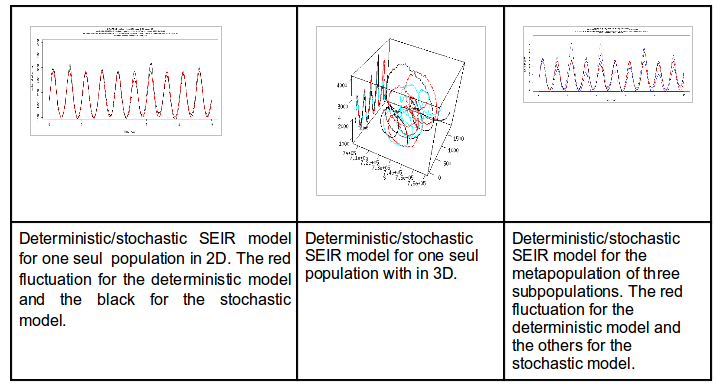
\includegraphics[width=0.3\textwidth]{smseir} \caption{Result of deterministic model and stochastic model with N=$10^{7}$,
$\mu=1/(70*365)$ per day, $\beta_{0}=1250/365$ day, $\beta_{1}=0.1$
day, $1/\sigma=8$days, $1/\gamma=5$ days, $\varphi=0$, simulation
time = 10 years. The red curve is for the deterministic model. The
black curve is for the stochastic model.}


\label{fig:smseirDETSTO} 
\end{figure}


The result (figure \ref{fig:smseirDETSTO}) is a good result. The
deterministic curve is so close to the stochastic model. This figure
points out that we have successfully transformed the deterministic
model to the sotchastic model.

Then, we simulate a metapopulation of three subpopulation with N=$10^{7}$.

\begin{figure}[tbph]
\centering 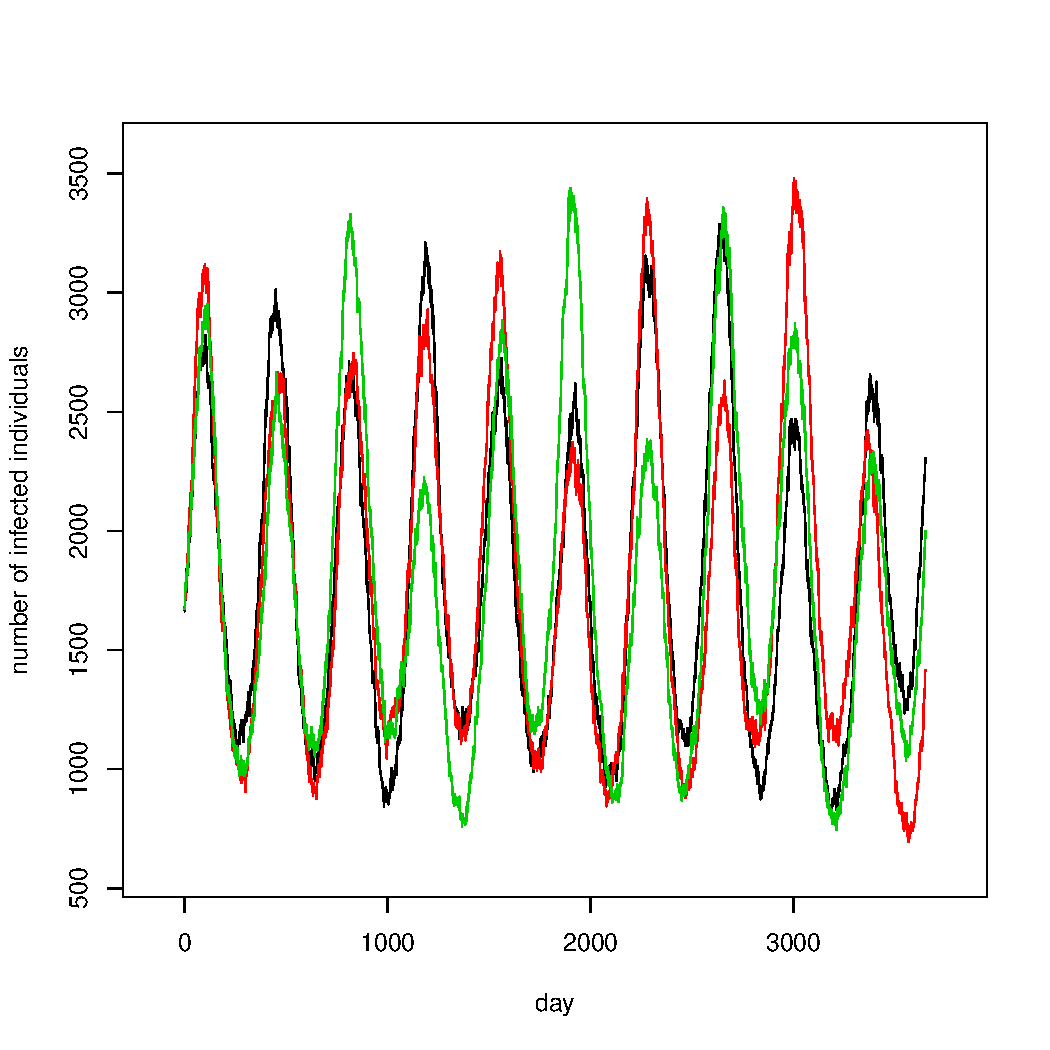
\includegraphics[width=0.3\textwidth]{smseirPOP3} \caption{Simulation of a metapopulation of three subpopulations with N=$10^{7}$,
$\mu=1/(70*365)$ per day, $\beta_{0}=1250/365$ per day, $\beta_{1}=0.1$
per day, $1/\sigma=8$ days, $1/\gamma=5$ days, $\varphi_{1}=\varphi_{2}=\varphi_{3}=0$
rad, coupling rate $\rho=0.0$ and simulation time = 10 years. The
curve of each subpopulation fluctuates very close to each other with
the same all values of parameters and initial availables.}


\label{fig:smseir} 
\end{figure}



\subsection{Global persistence in a metapopulation}

Here, we start exploiting the package \textquotedbl{}dizzys''. In
order to illustrate the interaction between disease transmissibility
and phase difference among subpopulations. We start this section by
studing the stochastic SEIR model in a metapopulation of $n$ subpopulations.
For this meta-population, we observe the disease extinction in time
due to spatial synchrony or spatial asynchrony that are influenced
by phase difference in seasonal forcing parameter. To create phase
difference, we change the value of the forcing phase for each city.
In this experience, we use a parameter $\varphi_{max}$ in radian
that runs in the interval from zero to $\pi$. With each value of
$\varphi_{max}$, based on \textbf{$n$} the number of subpopulations
in the metapopulation, we divide the interval {[}0, $\varphi_{max}${]}
into a set of (n-1) equal samples, so the value of the forcing phase
of the $i^{th}$ city is correspondent to $i^{th}$ value in the set.
We call $\varphi_{max}$ asynchrony parameter.

For our metapopulation of $n$ subpopulations, to do so we run first
$m$ independent simulations of our stochastic model. We calculate
then the average metapopulation size by summing subpopulations at
each sample time and averaging across the entire time series for each
metapopulation. Lastly, we record the dates $t$ of global disease
extinction in all these $m$ metapopulations. These dates allowed
to draw Kaplan-Meier survival curves from which we estimated the extinction
rate $\chi$: 
\begin{equation}
M(t)=\exp(-\chi t)
\end{equation}
 where $M(t)$ ($0\leqslant M(t)\leqslant m$) is the number of metapopulations
in which the disease is not extinct at time $t$. The extinction rate
$\chi$ is reparameterized in terms of predictor variables and regression
parameters. Here, we reparameterize$\chi$ with $\chi=exp(-pt)$ where
$p$ is the coefficient that characterizes the probability of the
global disease persistence.

To estimate the persistence coefficient, here, we use the survival
regression model (R package '$survival$' \cite{survival-package}).
For that, we find the persistence coefficient of the number of metapopulations
in which the disease is extinct in time. According on this persistence
coefficient, we study the relation between the global persistence
and its level of synchrony due to the phase of the forcing.


\subsubsection{Global persistence and time}

Here, we start with a simplest metapopulation of two subpopulation.
We have $N_{1}=N_{2}=300,000$, the rate of coupling $\rho=0.01$,
the simulation time 50 years, the number of simulations $m=100$,
and $\varphi_{max}=\{0,\pi/2,\pi\}$. We have three Kaplan-Meier survival
curves for each value of $\varphi_{max}$ as figure \ref{fig:persm100phi0pi2pi_01}.

\begin{figure}[tbph]
\centering 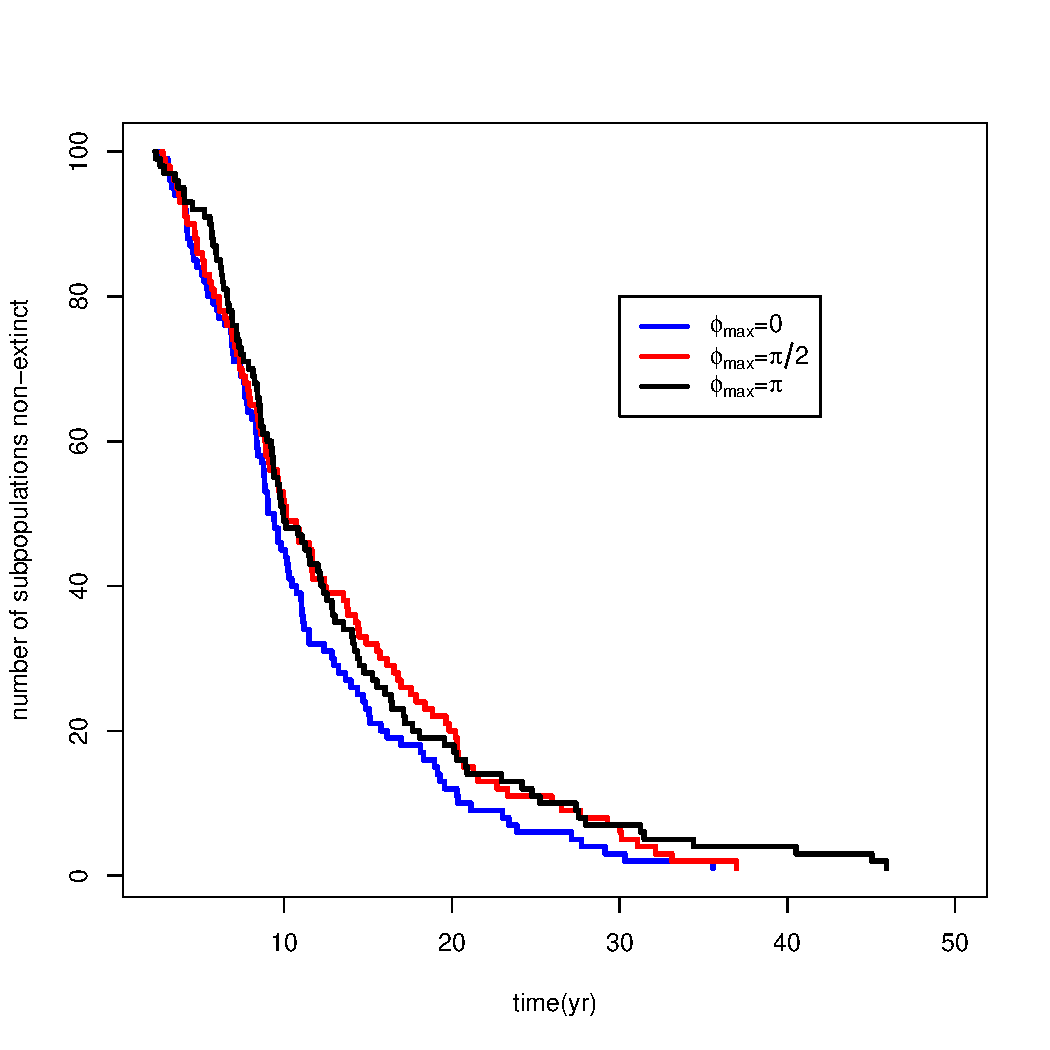
\includegraphics[width=0.3\textwidth]{smRep100Vil02R001N3e5}
\caption{Kaplan-Meier survival curves for disease persistence after 100 different
simulation, with N=300000, $\mu=1/(70*365)$ per day, $\beta_{0}=1250/365$
per day, $\beta_{1}=0.1$ per day, $1/\sigma=8$ days, $1/\gamma=5$
days, coupling rate $\rho=0.01$. \protect \protect \protect \\
Disease persistence time after 100 simulations of $\varphi_{max}=0$
rad, $\varphi_{max}=\pi/2$ rad and $\varphi_{max}=\pi$ rad. The
blue survival curve for $\varphi_{max}=0$, the red survival curve
for $\varphi_{max}=\pi/2$ and the black curve for $\varphi_{max}=\pi$.
The persistence time of $\varphi_{max}=0$ is the shortest. The persistence
time of $\varphi_{max}=\pi$ is the longest.}


\label{fig:persm100phi0pi2pi_01} 
\end{figure}


The phase of forcing of the $subpopulation_{1}$ is always fixed $0$,
but this of the $subpopulation_{2}$ increases from $0$ to $\pi$.
It means that, in the first experience, $\varphi_{max}=0$, the two
subpopulations are in synchrony with all beginning conditions. The
disease persistence time is the shortest. Then, the two subpopulations
become asynchrony when $\varphi_{max}=\pi/2$ or $\pi$. The symmetry
of fixed points is just broken at the starting moment. It is reason
for that the level of synchrony of the metapopulation decreases. Additionally,
we find that the value of the asynchrony parameter $\varphi_{max}$
change according to increasing tendency, the phase difference between
the fluctuations of the two infection rates $\beta$ increases also,
and the global persistence time in the metapopulation thus augments.
When \textbf{$\varphi_{max}=\pi$, }the two subpopulations are in
antiphase. This is the most difficult case to find global extinction,
the persistence time is the longest. In short, the level of synchrony
between subpopulation is stronger, metapopulation is easier to find
global extinction. Make all subpopulations synchronize is the easiest
way at which disease goes to extinct.


\subsubsection{Estimating global persistence coefficient when $\varphi_{max}$ alters}

In this part, the Kaplan-Meier survival curve of the global disease
persistence time in a metapopulation for each value $\varphi_{max}$
is considered as a parameter that is called global persistence coefficient
of that $\varphi_{max}$. Depending on the base of the persistence
time caused by the phase difference in the metapopulation of two subpopulations,
we are going to exploit metapopulations of many subpopulations. We
use survival functions to estimate this global persistence coefficient
with confidence interval 95\%. The result is shown as following figure
\ref{fig:perrateVil8}.

\begin{figure}[tbph]
\centering 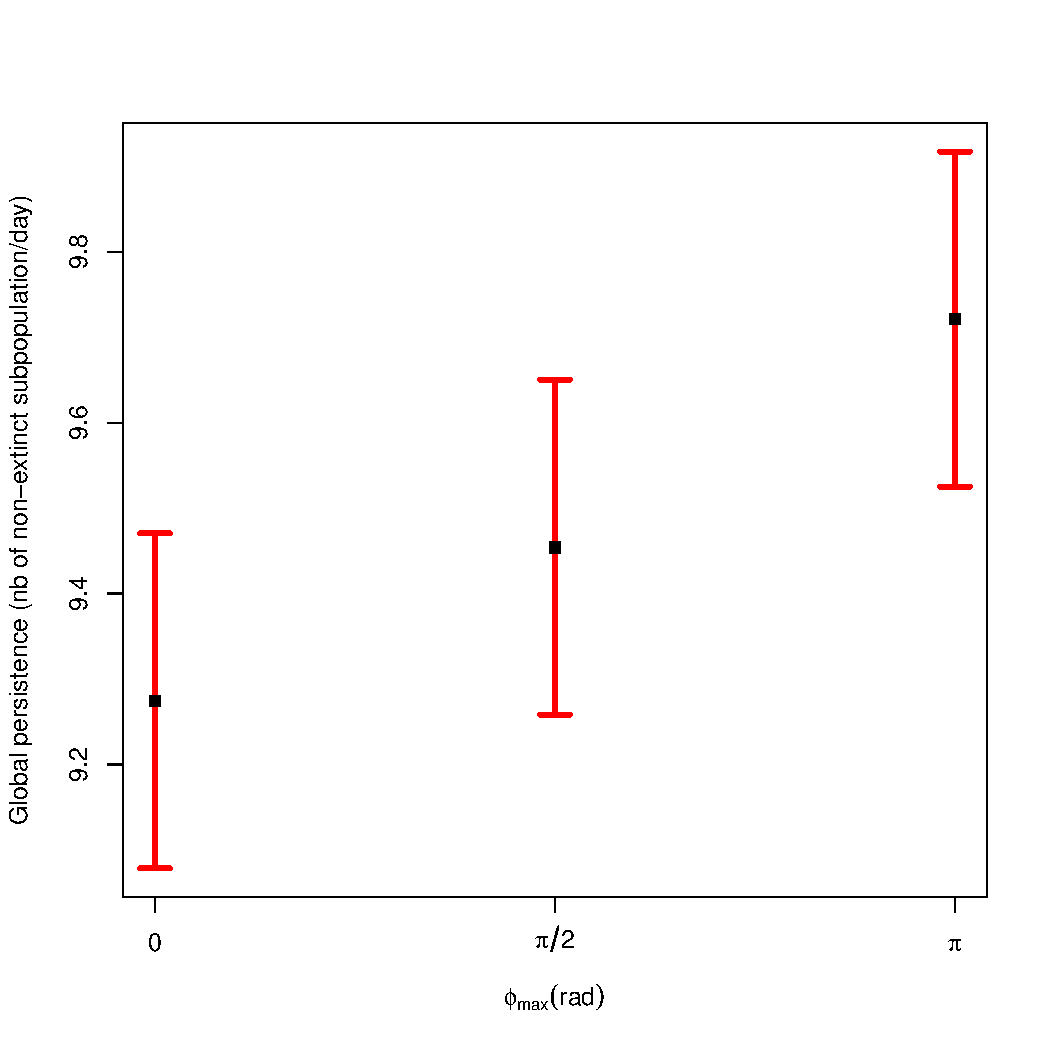
\includegraphics[width=0.3\textwidth]{resMetaPop08N3e5Rho01Rep100}
\caption{Estimated coefficient of global disease persistence in the metapopulation
of eight subpopulations after 100 different simulations N=3{*}$10^{5}$,
coupling rate $\rho=0.1$. Here, with 95\% confidence interval, these
intervals are limited by lower and upper confidence limits.}


\label{fig:perrateVil8} 
\end{figure}


This figure \ref{fig:perrateVil8} points out to us that the distance
of the estimated scales is quite far to each other. The persistence
probability rises when $\varphi_{max}$ runs from $0$ to $\pi$.
The phase difference strongly influences both disease persistence
time and global disease persistence probability. The asynchrony between
subpopulations is the main reason to respond very familiar question
why has the infectious disease been never extinct.


\subsubsection{Influence of demographic parameters on persistence of infectious
diseases}


\paragraph*{Population size of subpopulation}

In the metapopulation of 06 subpopulations, we implement experiences
with different population sizes of subpopulation. We performe 100
different simulation for the metapopulation of 06 subpopulations in
which all subpopulation has the same population size N. We set N from
5000 to 500000 individuals. The result (Figure \ref{fig:effectPOPsize})
affirms that the population size influences strongly the global persistence
time of an infectious disease in a metapopulation. The number of individuals
in a subpopulation increases, so the global persistence probability
increases also.

\begin{figure}[tbph]
\centering 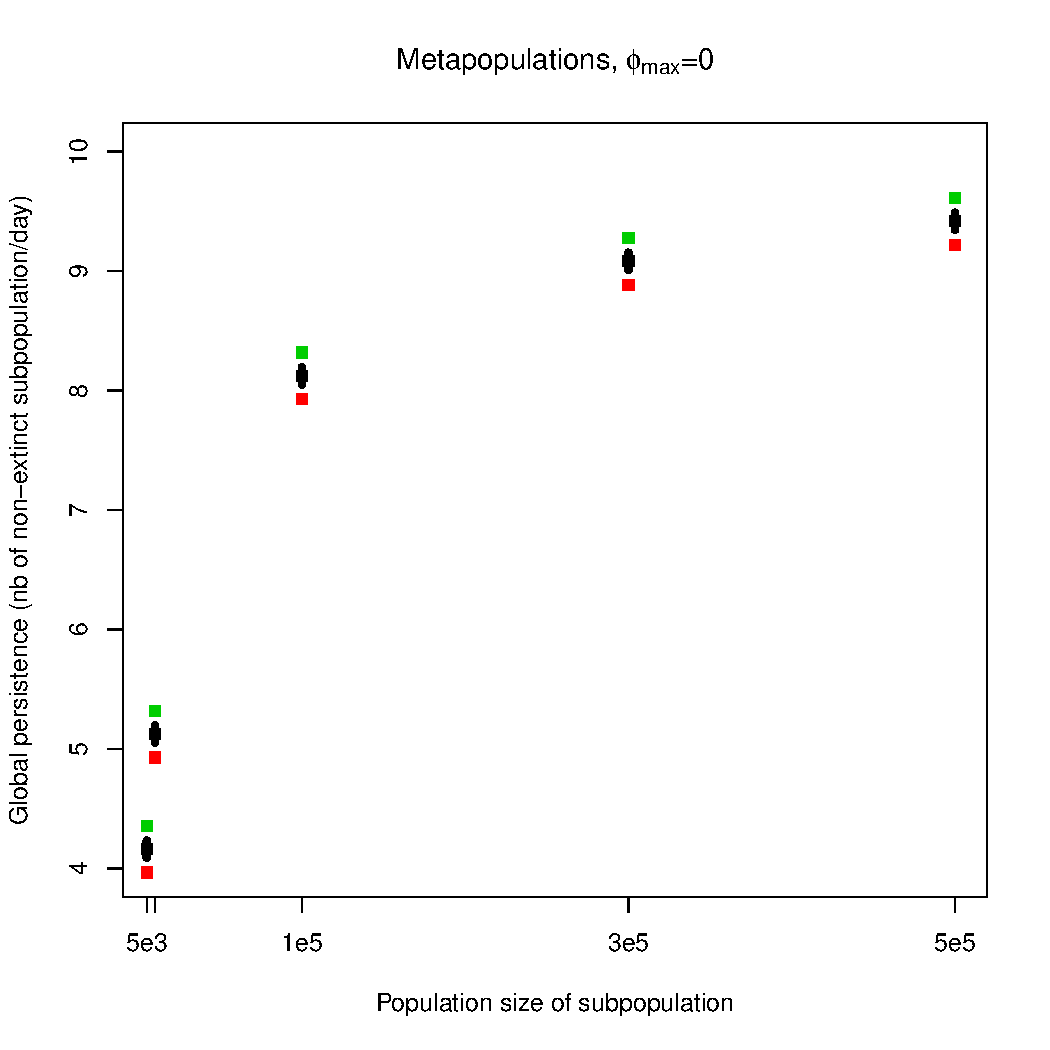
\includegraphics[width=0.4\textwidth]{resMeta06rho01NChangephi0}
\caption{Estimated persistence coefficient in the metapopulation of six subpopulations
after 100 different simulations. The population size of subpopulation
is in the set \{5000, 10000, 1e5, 3e5, 5e5\}. Here, with 95\% confidence
interval, these intervals are limited by lower and upper confidence
limits.}


\label{fig:effectPOPsize} 
\end{figure}



\paragraph*{Number of subpopulation in a metapopulation}


\paragraph{\textmd{In addition to the result of the population size, here we
are going to explore influence of the number of subpopulation in a
metapopulation on disease persistence of this metapopulation. We set
first all metapopulation is the same population size $N=10^{5}$ and
$\varphi_{max}=\pi$, then we change the number of subpopulation in
metapopulation from three to 30. We obtain the same result as when
the population size augments. The persistence probability scales directly
the number of subpopulation in a metapopulation. }}

\begin{figure}[tbph]
\centering 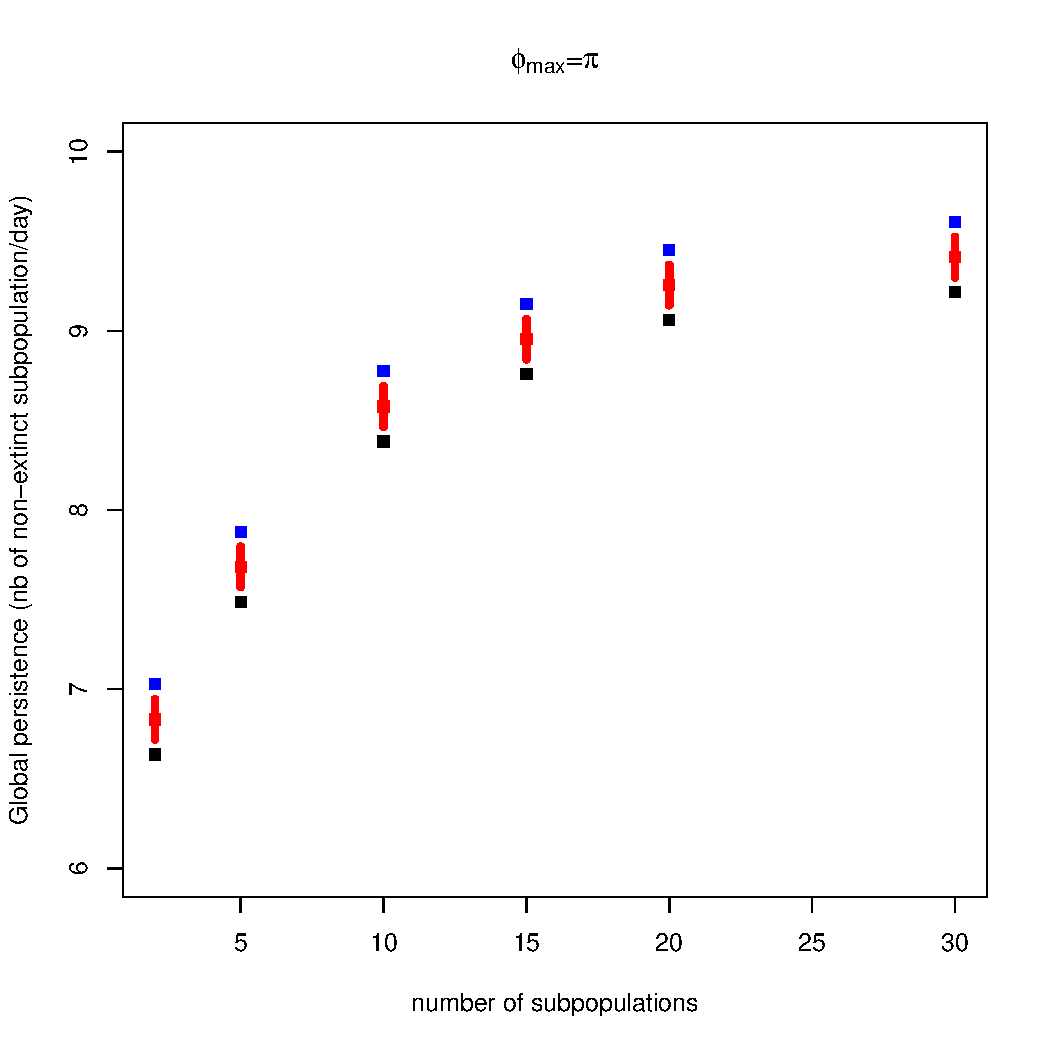
\includegraphics[width=0.3\textwidth]{/home/tran/Bureau/miparcours/resMetaPop35710152030N1e5Rho0001Rep100}
\caption{Estimated persistence probability in the metapopulation of multi-subpopulations
after 100 different simulations. The number of subpopulations alters
in the set \{2, 5, 10, 15, 20, 25, 30\}. Here, with 95\% confidence
interval, these intervals are limited by lower and upper confidence
limits. }


\label{fig:effectNbPOP} 
\end{figure}



\paragraph*{Coupling force }

According to Keeling(2008), due todispersal rate $\rho$, the persistence
time of metapopulation is considered as a function of dispersal rate.
In order to affirm this supposition, here we change coupling rate
from weak to strong in a metapopulation of five subpopulations with
the population size of each subpopulation $N=10^{5}$. The dispersal
rate $\rho$ is divided into three intervals. These are low, intermediate
and high coupling rate intervals. In each interval, we choose some
coupling rates that highlight the coupling strength among subpopulations
in metapopulation. We have the result as follows (figure \ref{fig:couplingPop05}).

\begin{figure}[tbph]
\centering 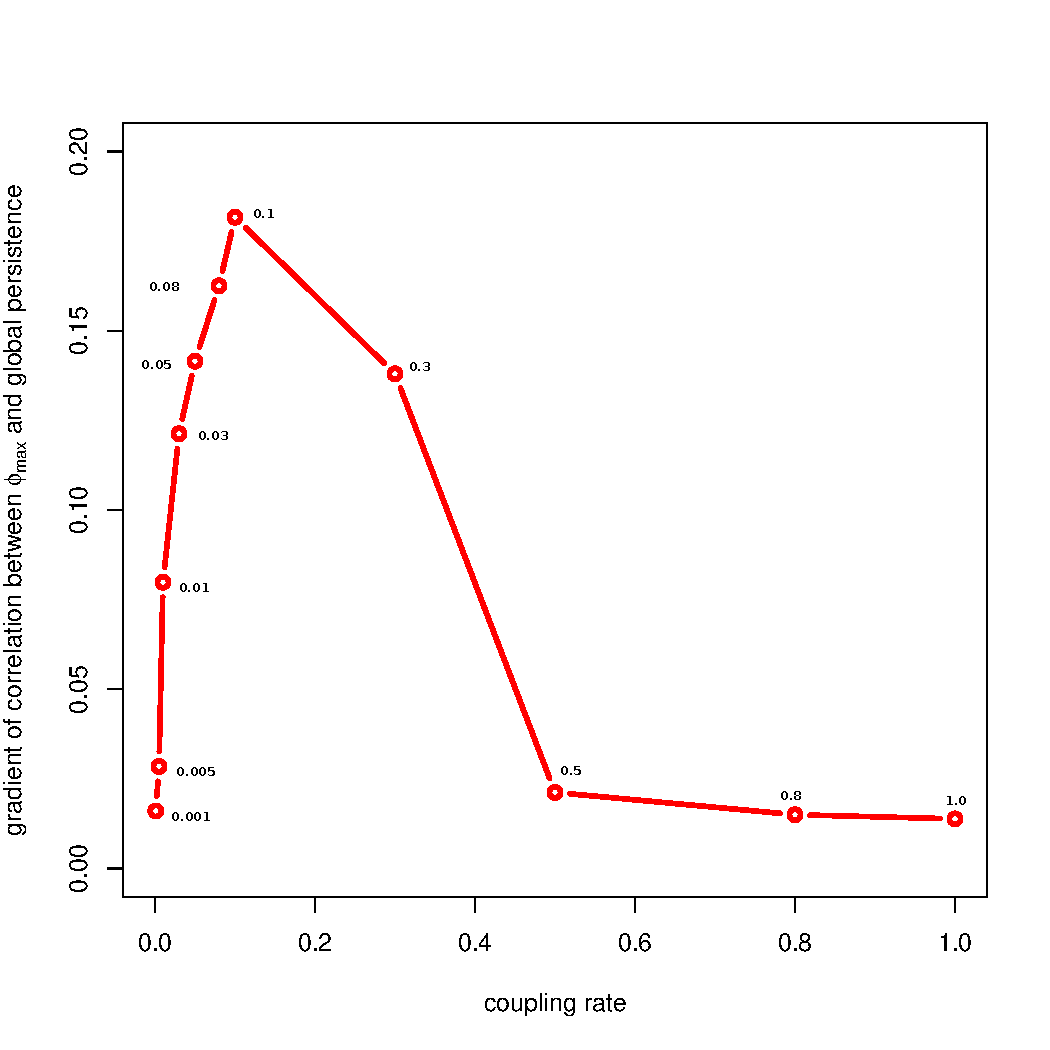
\includegraphics[width=0.3\textwidth]{resPenteVil05multiRho}
\caption{Correlation between coupling rate and gradient of level of synchrony
and persistence probability in the metapopulation of five subpopulation.
Here, the coupling rate $\rho$ is in ${0.0001,0.0005,0.001,0.003,0.008,0.01,0.03,0.05,0.08,0.1,0.3,0.5,0.8,1}$,
the level of asynchrony $\varphi_{max}$ in ${0,\ensuremath{\pi/2},\ensuremath{\pi}}$
and the population size of each subpopulation N=$10^{5}$.}


\label{fig:couplingPop05} 
\end{figure}


When the coupling rate is small from 0.0001 to 0.008, the gradient
of the correlation between $\varphi_{max}$ and persistence probability
increases very slowly. However, the persistence probability augments
in a sudden way when the coupling rate changes from 0.008 to 0.1.
Lastly, the gradient strongly decreases when the coupling rate is
so robust from 0.5 to1. Based on this figure, the disease persistence
coefficient is one humped function for the coupling rate. The medium
coupling rate (from 0.005 to 0.1) maximizes disease persistence in
metapopulation.


\section{Conclusion and perspective}

We successfully built a version for the susceptible-infected-recovered
stochastic metapopulation model. The infection rate $\lambda_{i}$
for $subpopulation_{i}$ portrayed all effects inside as well as outside
on disease transmission chain between individuals in the same subpopulation
or among subpopulations. Moreover, our metapopulation model became
more detailed when we brought seasonality in metapopulation model
to create periodic transmission in year that here highlights seasonal
change as well as school period of children. We have metapopulation
model with different contact rates. This is more complex model than
any used metapopulation model. We sketched successfully in-phase and
sometime out-of-phase (“antiphase'') models across suburbs of He's
2003 \cite{He2003}. In addition, the results about the persistence
of infectious diseases are in agreement Rozhnova(2012) \cite{Rozhnova2012},
Heino in 1997 \cite{Heino1997}, Huffaker(1958) \cite{huffaker1958experimental},
Holyoak and Lawler(1996) \cite{holyoak1996persistence}, and Yaari
et al. (2012) \cite{Yaari2012} when they exhaustively explored the
disease persistence behavior of many different metapopulation models. 

In order to continue my thesis, we will exploit the global persistence
and the disease transmission among subpopulations under a new shape
of metapopulation in epidemiology. It is the gravity model in epidemiology.
This model is a very simple model, and can be used to explain the
spatial epidemiologic dynamics. We says it simply that the strength
of coupling between any two populations depends on the size of these
two populations and the distance between them (so this model is quite
similar to Newton's law of universal gravitation, the attraction between
two bodies depends on the masses of the bodies and the distance between
the bodies). In epidemiology, we will call the “mass” the population
size. Then, we set a gravity metapopulation model with the different
positions and the different population sizes of subpopulations. Finally,
we will exploit the disease transmission in the gravity metapopulation
model.

One more main work in my thesis, it is the optimization of the vaccination
policies. We set it in the last part of my thesis, because first of
all, we must deeply exploit the actual nature of the infectious disease
transmission in the different disease model, then we are going to
have a good vaccination policy for a metapopulation.


\section*{Manuscript :}

T.C.G. Tran, J.D. Zucker, M.Choisy, Quantifying the effect of synchrony
on the persistence of infectious diseases in a metapopulation.

 \bibliographystyle{plain}
\bibliography{bib_art_Pers,bikBokEpidemics,bikCCS}


{[}17{]} http://microbiology.mtsinai.on.ca/faq/transmission.shtml

{[}18{]} http://en.wikipedia.org/wiki/Epidemic\_model 
\end{document}
